%!TEX root = ../Manuale.tex
%%--------------------------------------------------------------------------
%% ALLARMI
%%--------------------------------------------------------------------------



\chapter{Alarms}
On a smartphone the section dedicated to alarms is mainly composed of a list; selecting an item opens a second screen containing the details of the alarm selected. On a tablet these two screens are combined into one. \\ 
In the details of the alarm is possible to navigate the map preview or enlarge it to full screen by tapping the appropriate button. Touching the MAC address of the device that generated the alarm shows a card with the details of the device; selecting the appropriate item from the overflow menu shows the current device position on the map.

	\begin{figure}[h!]
		  \centering
		    \centering{%
		      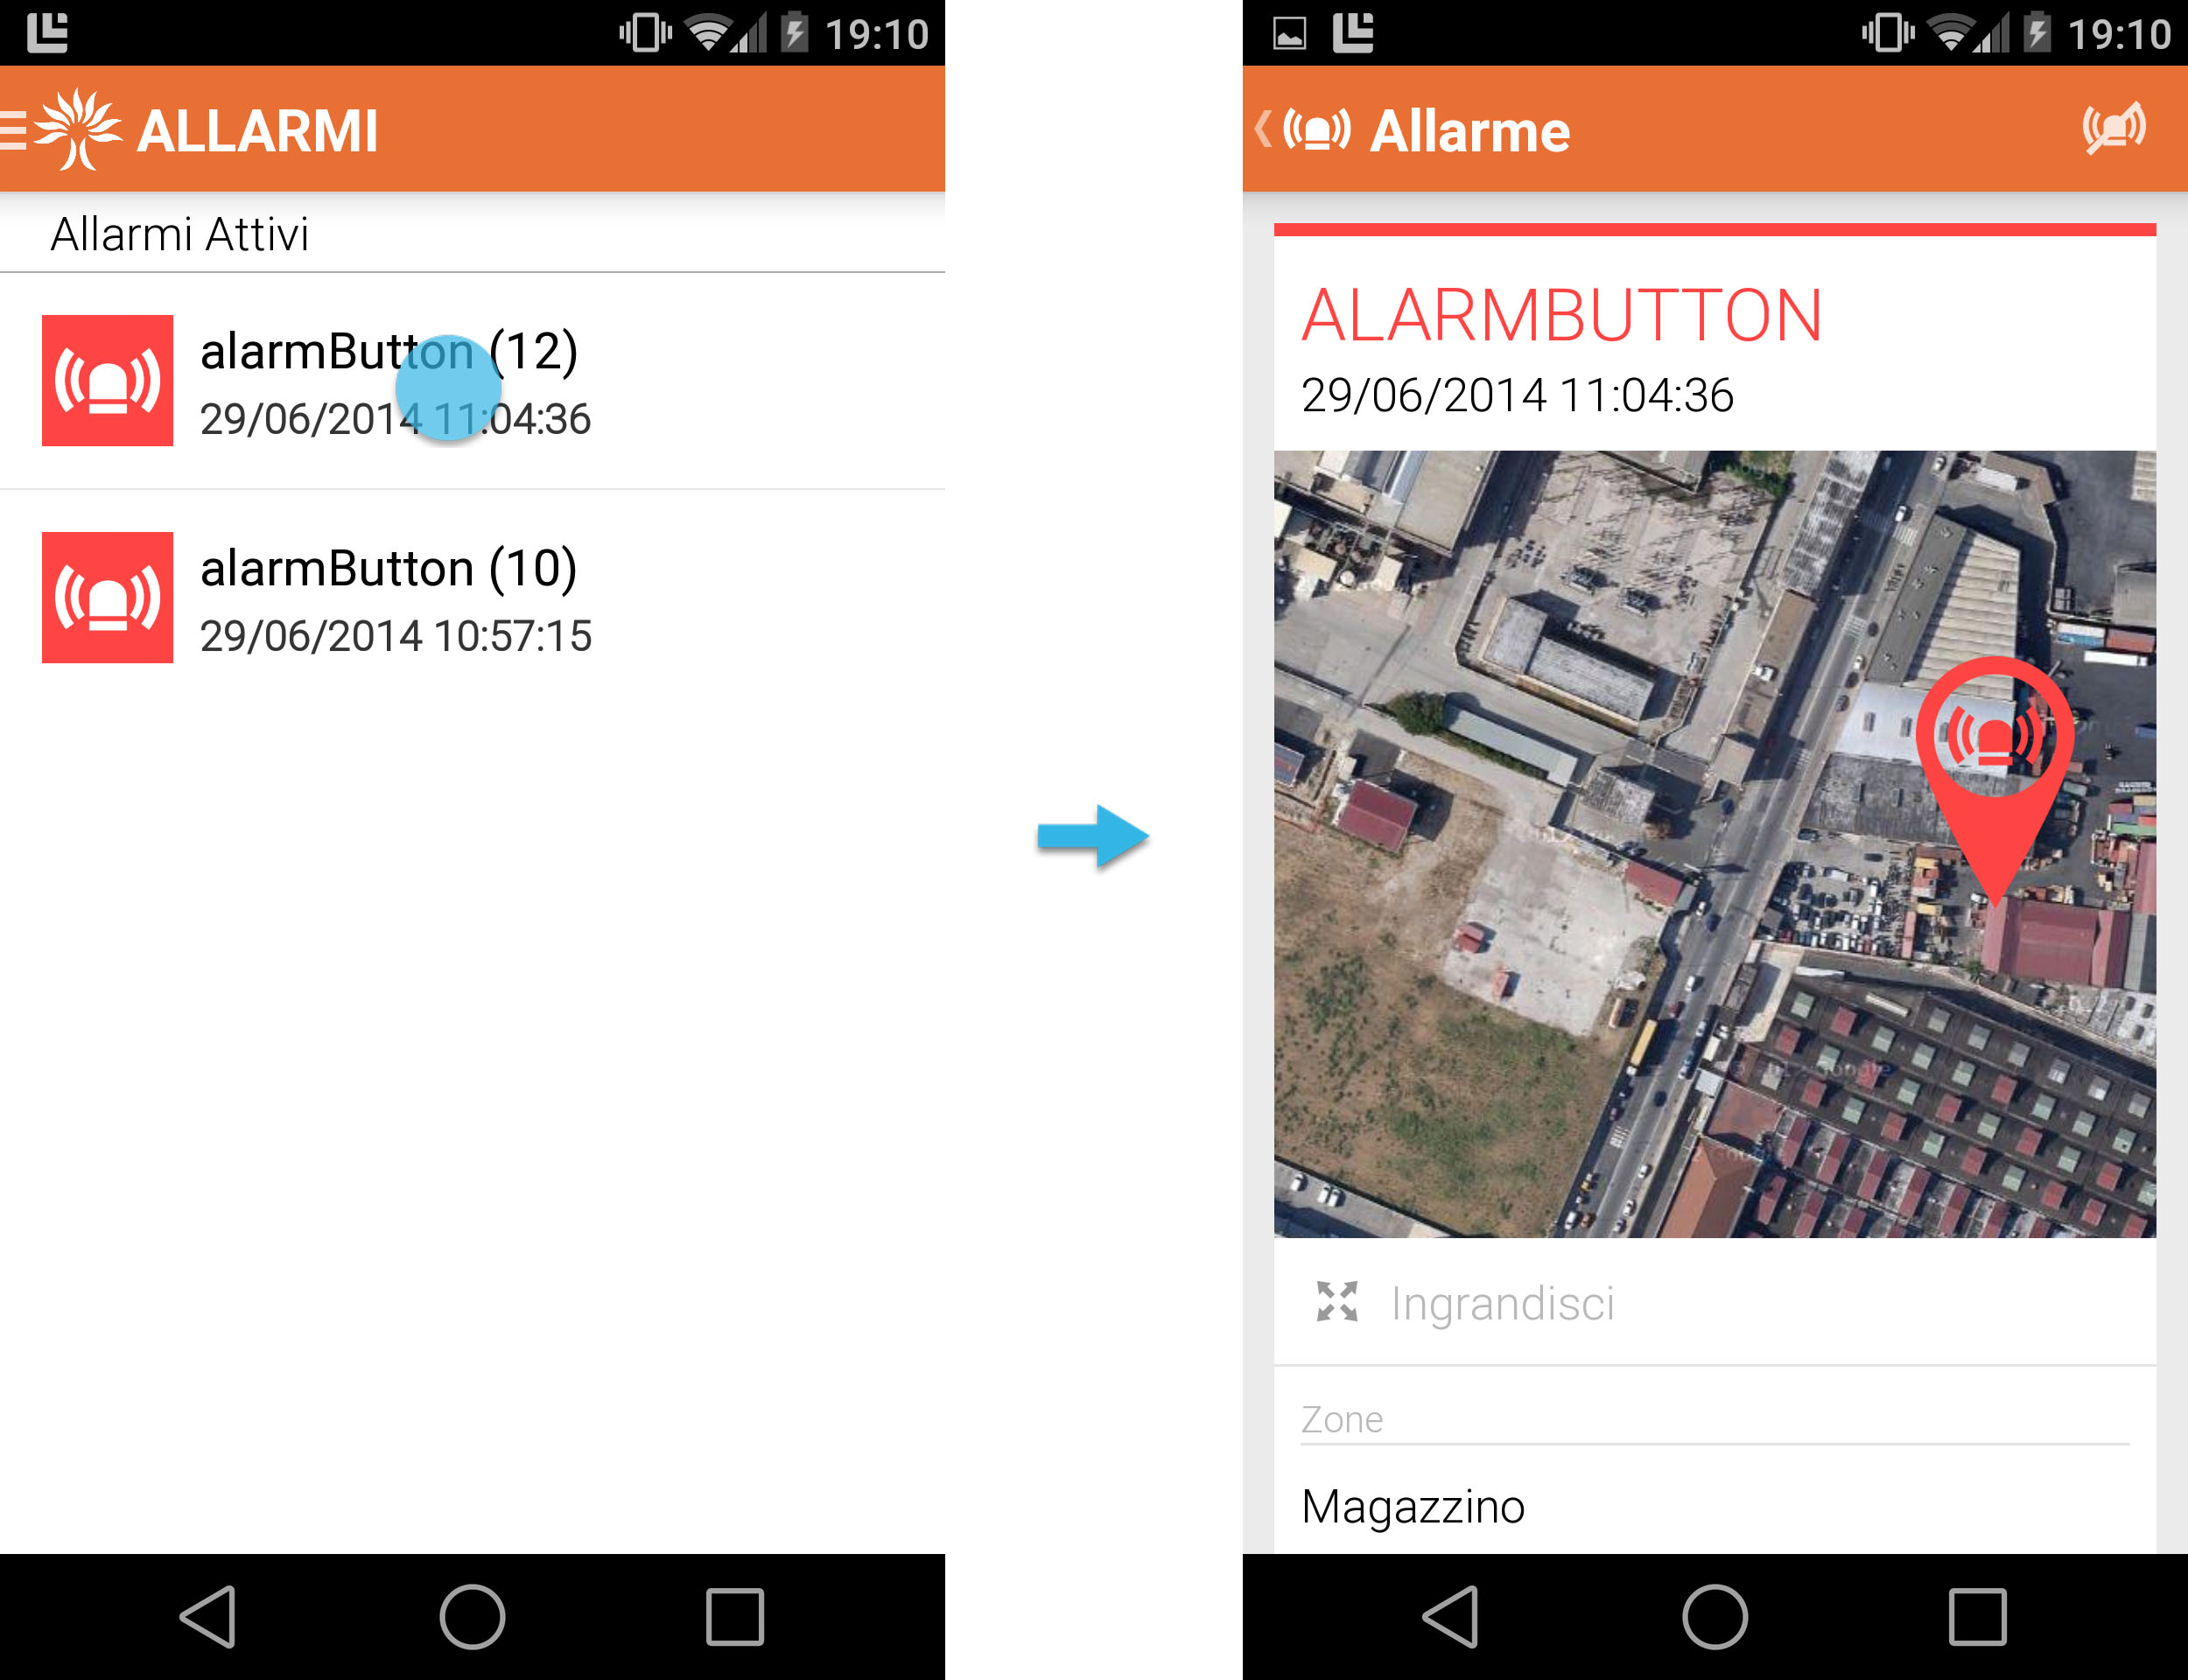
\includegraphics[width=0.8\textwidth]{phone_allarmi_dettagli.jpg}}
		  \caption{Phone - Alarm details}
	\end{figure}

	\begin{figure}[h!]
		  \centering
		    \centering{%
		      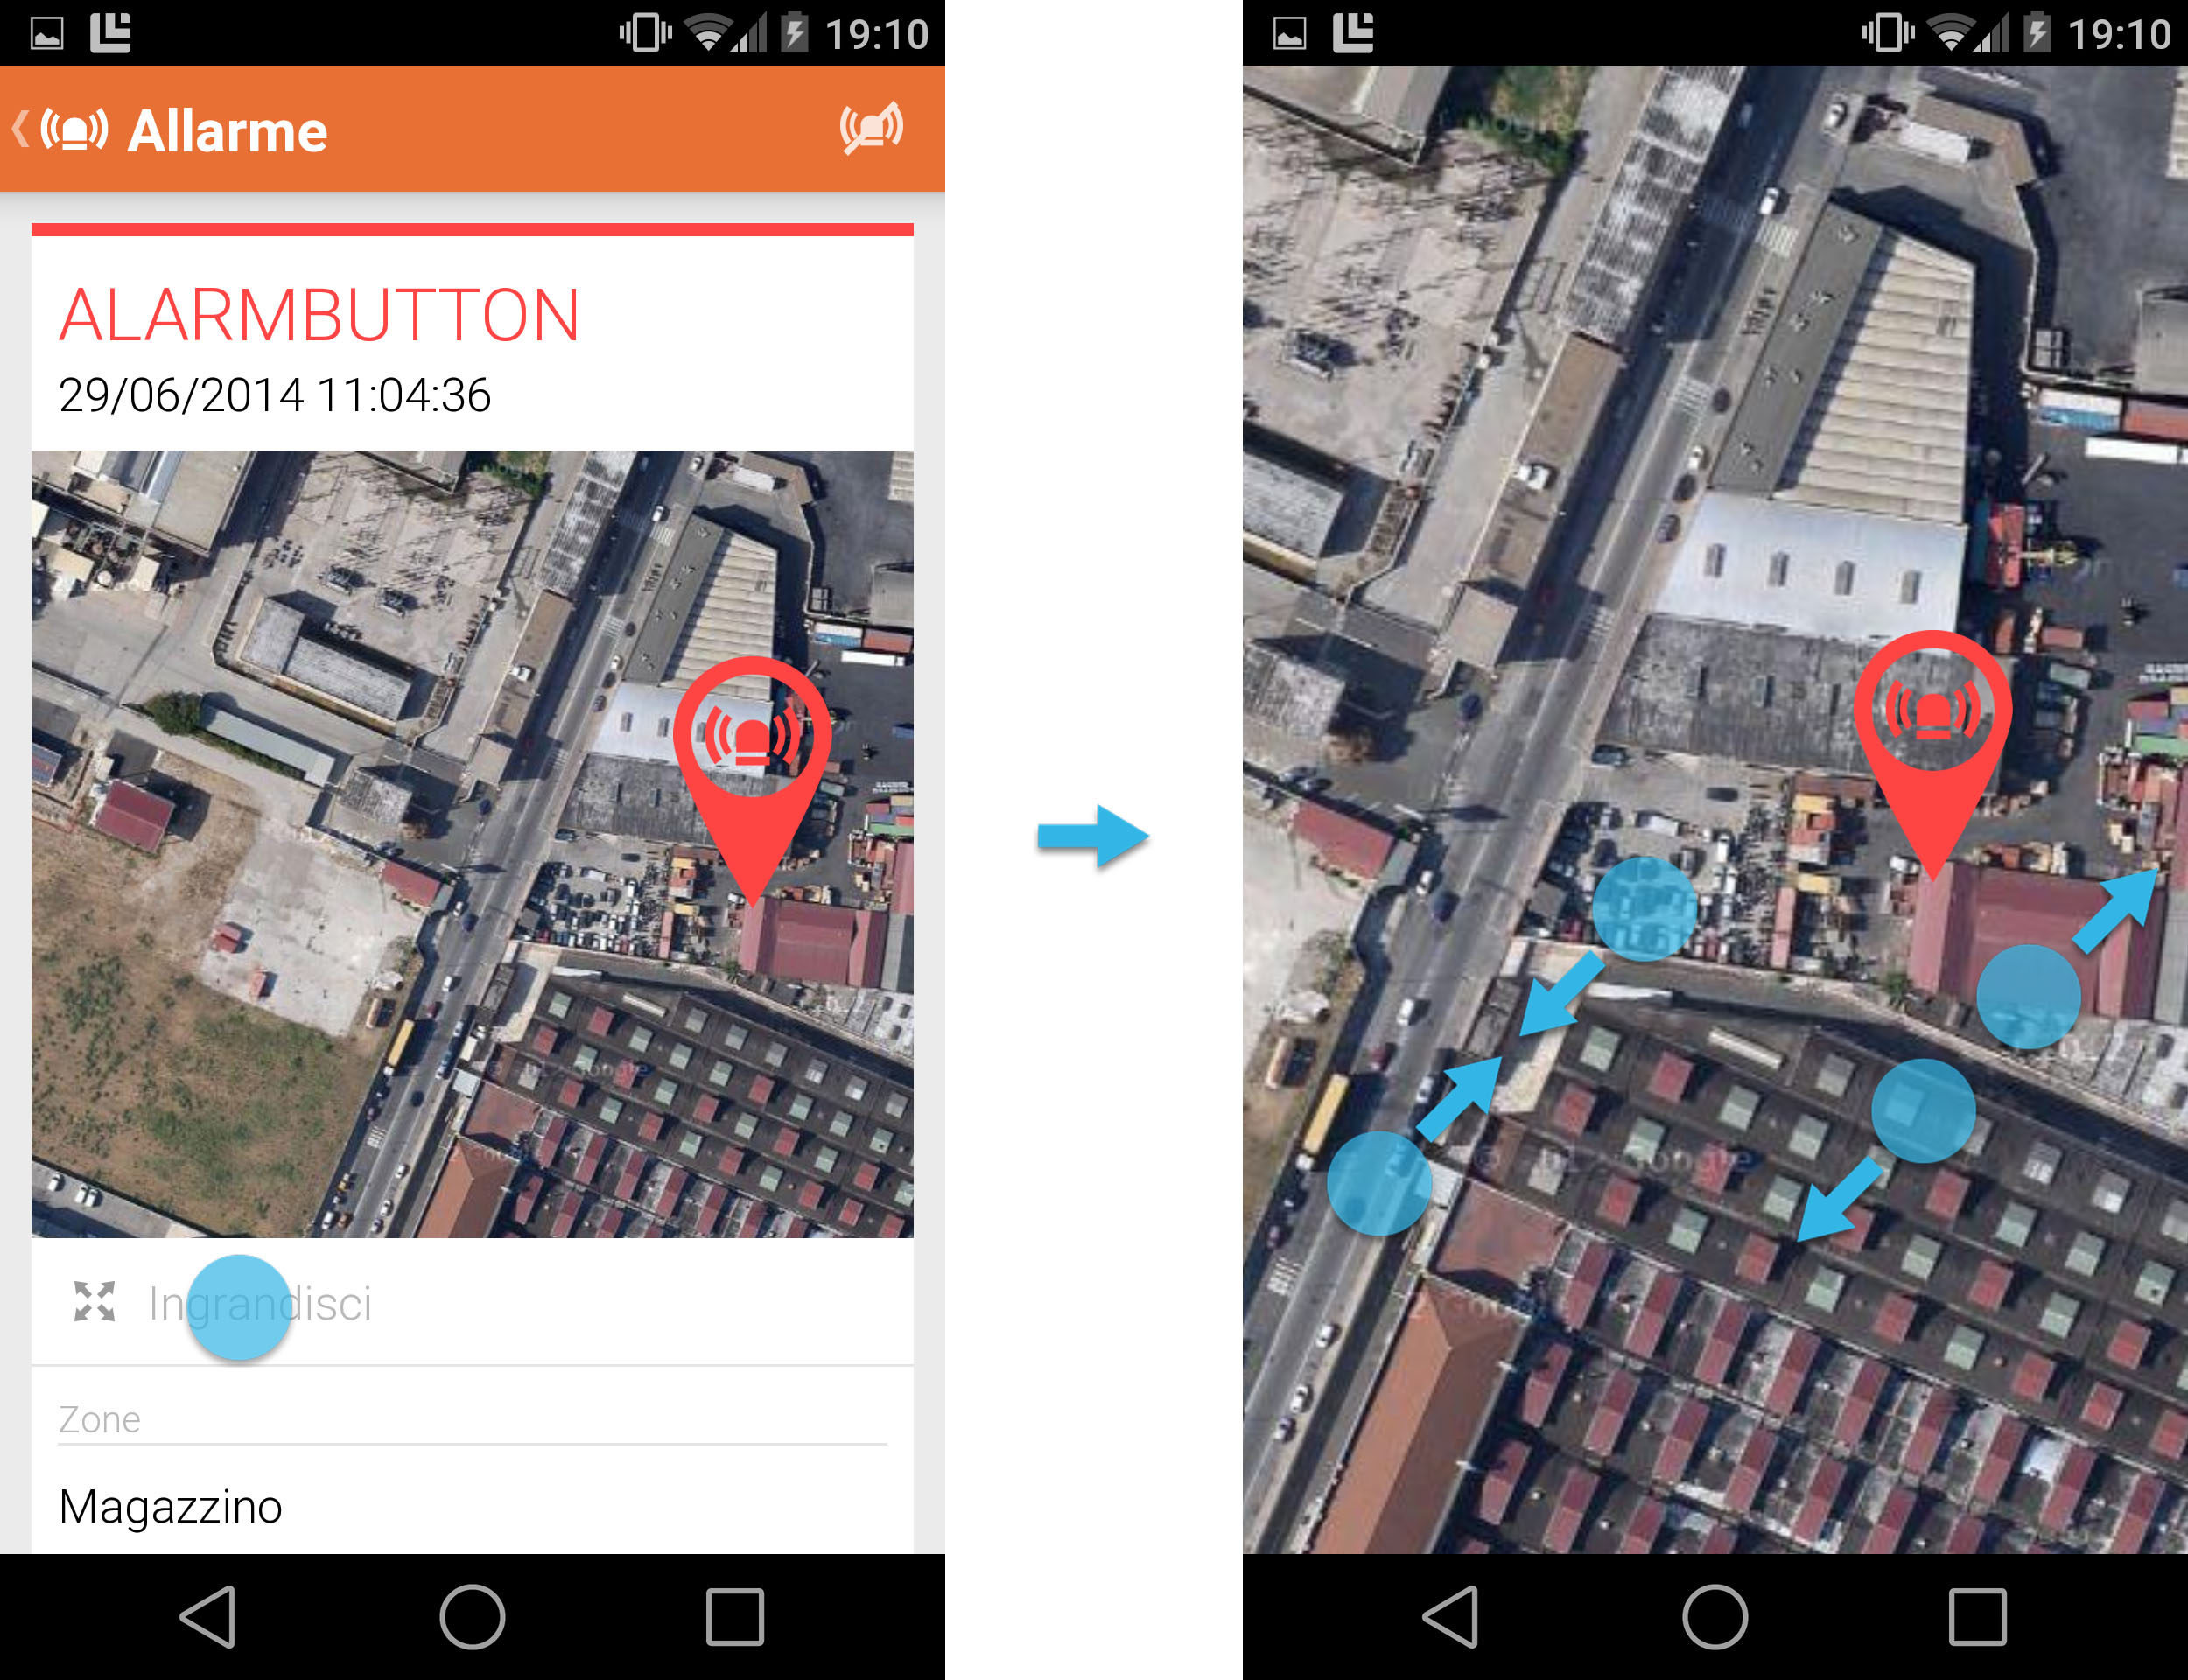
\includegraphics[width=0.8\textwidth]{phone_allarme_map.jpg}}
		  \caption{Phone - Map zoom}
	\end{figure}

	\begin{figure}[h!]
		  \centering
		    \centering{%
		      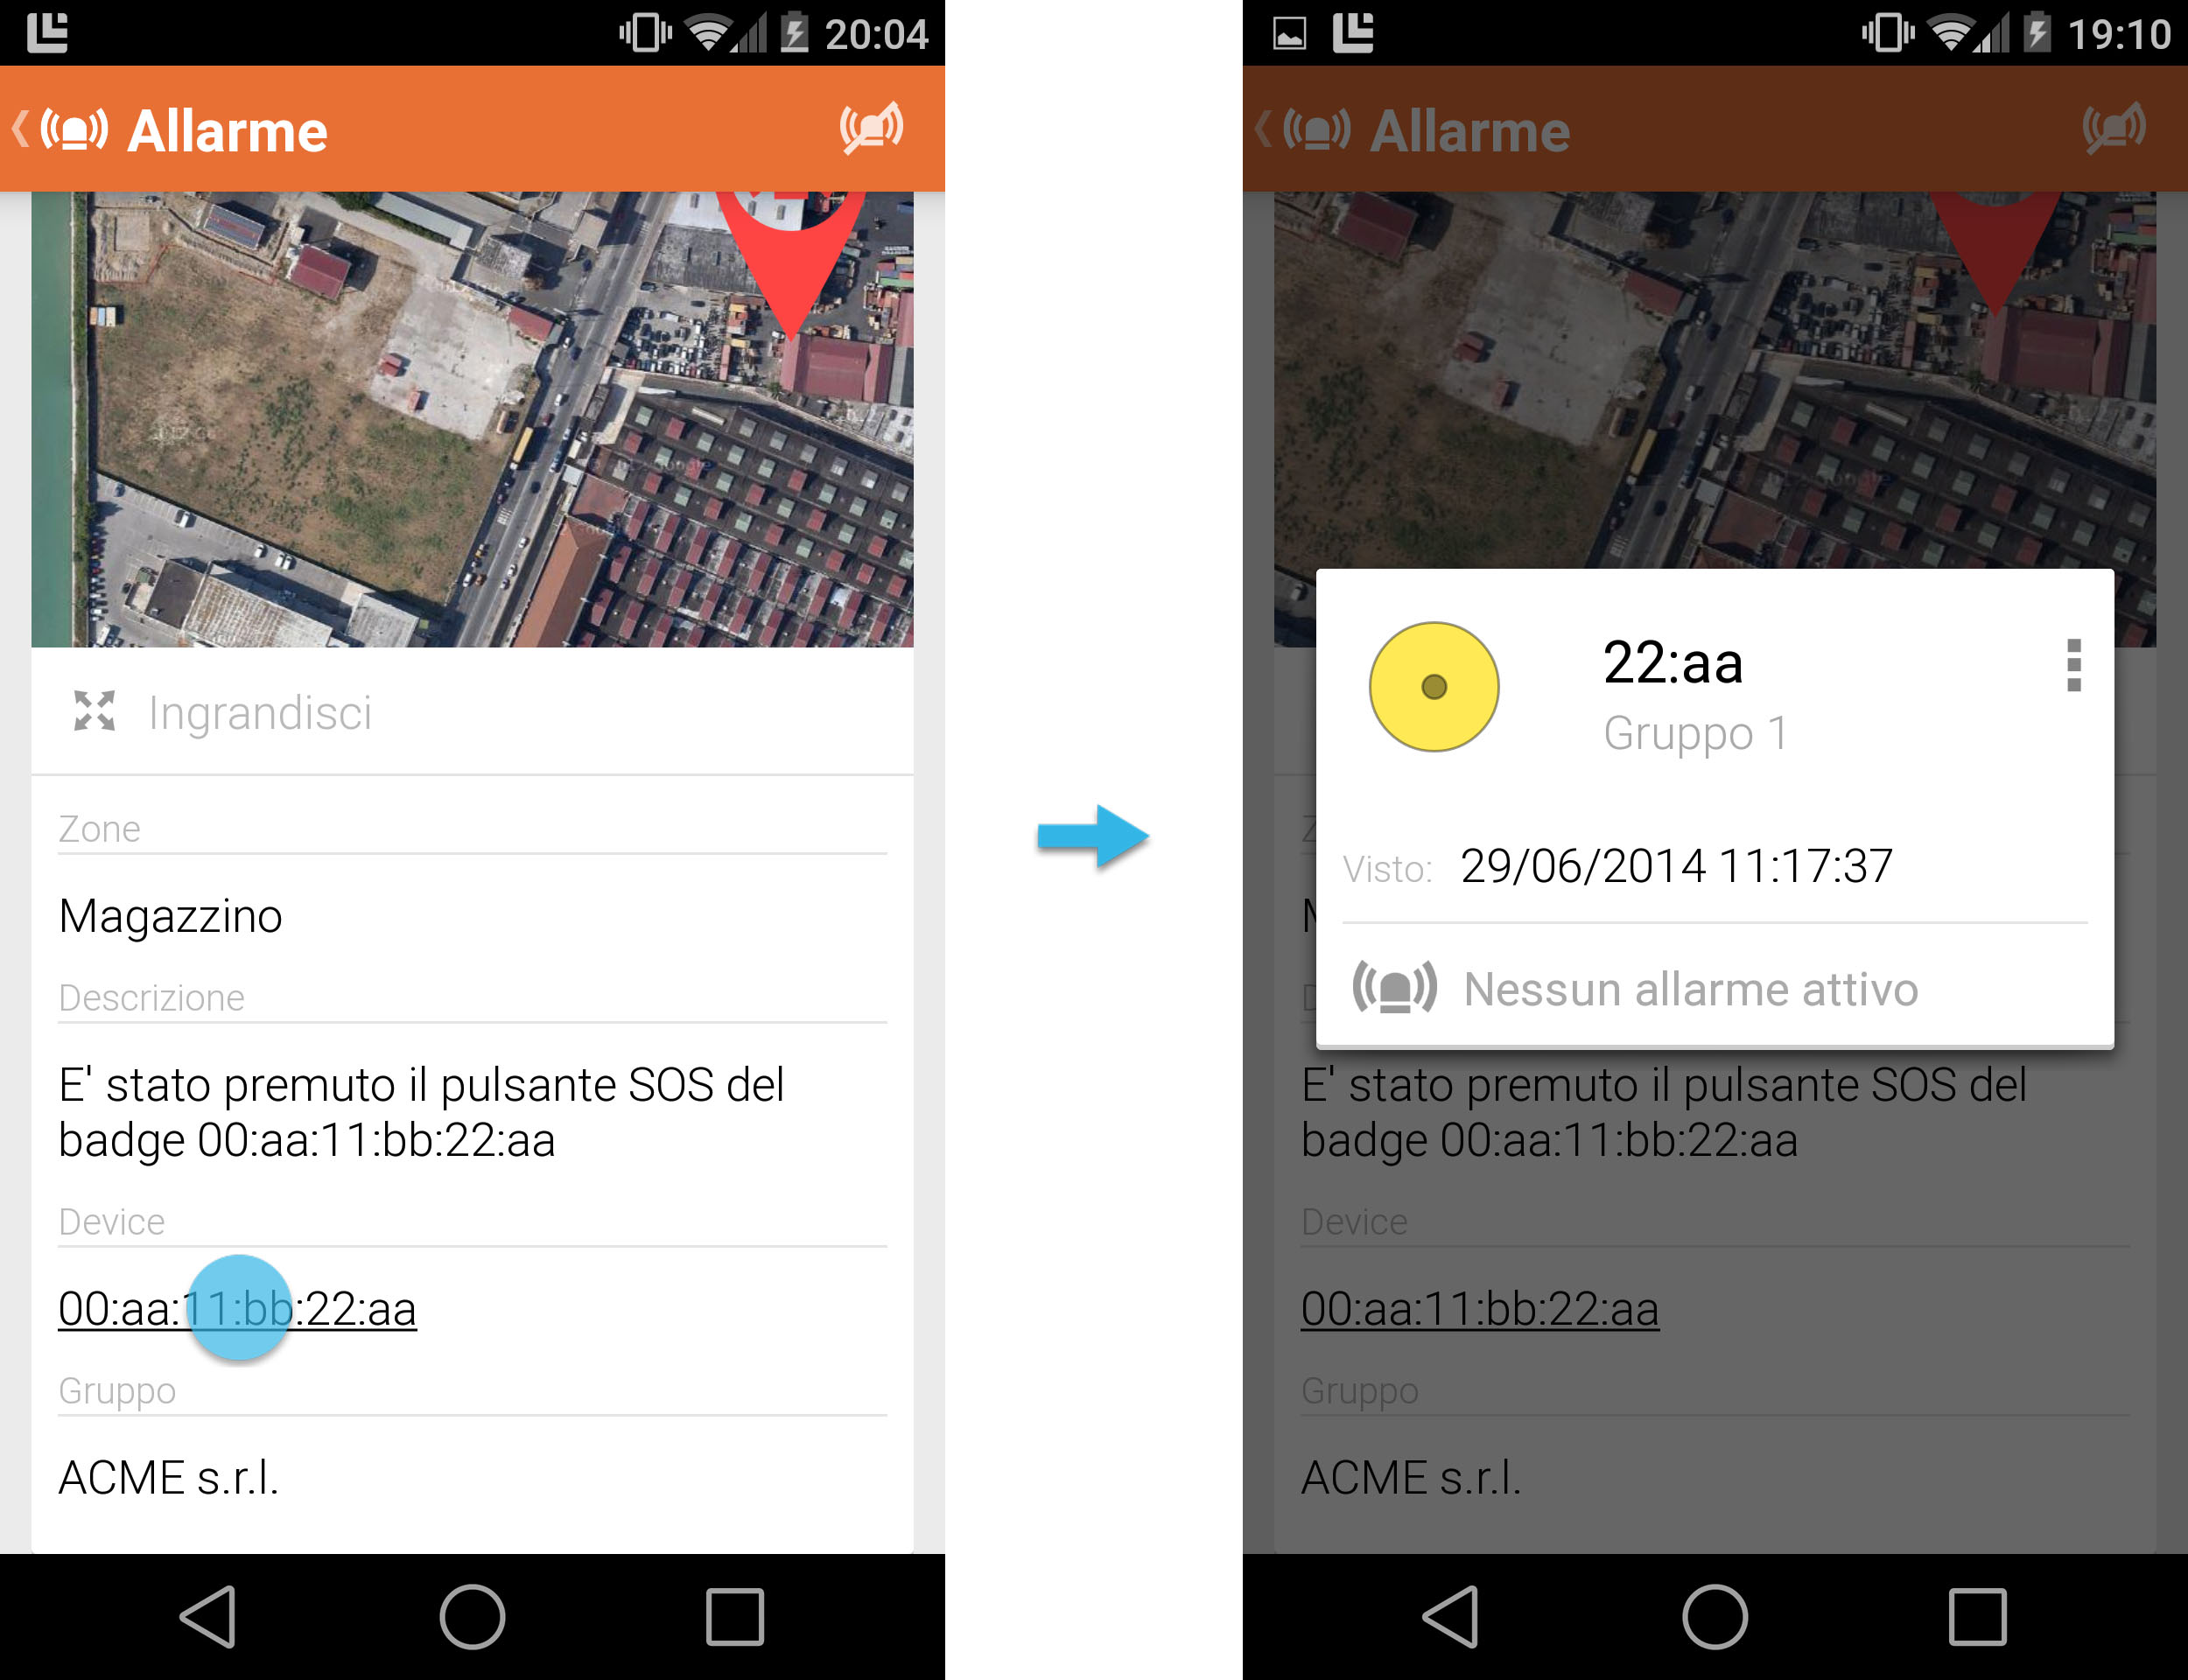
\includegraphics[width=0.8\textwidth]{phone_allarme_device.jpg}}
		  \caption{Phone - Device details}
	\end{figure}

	\begin{figure}[h!]
		  \centering
		    \centering{%
		      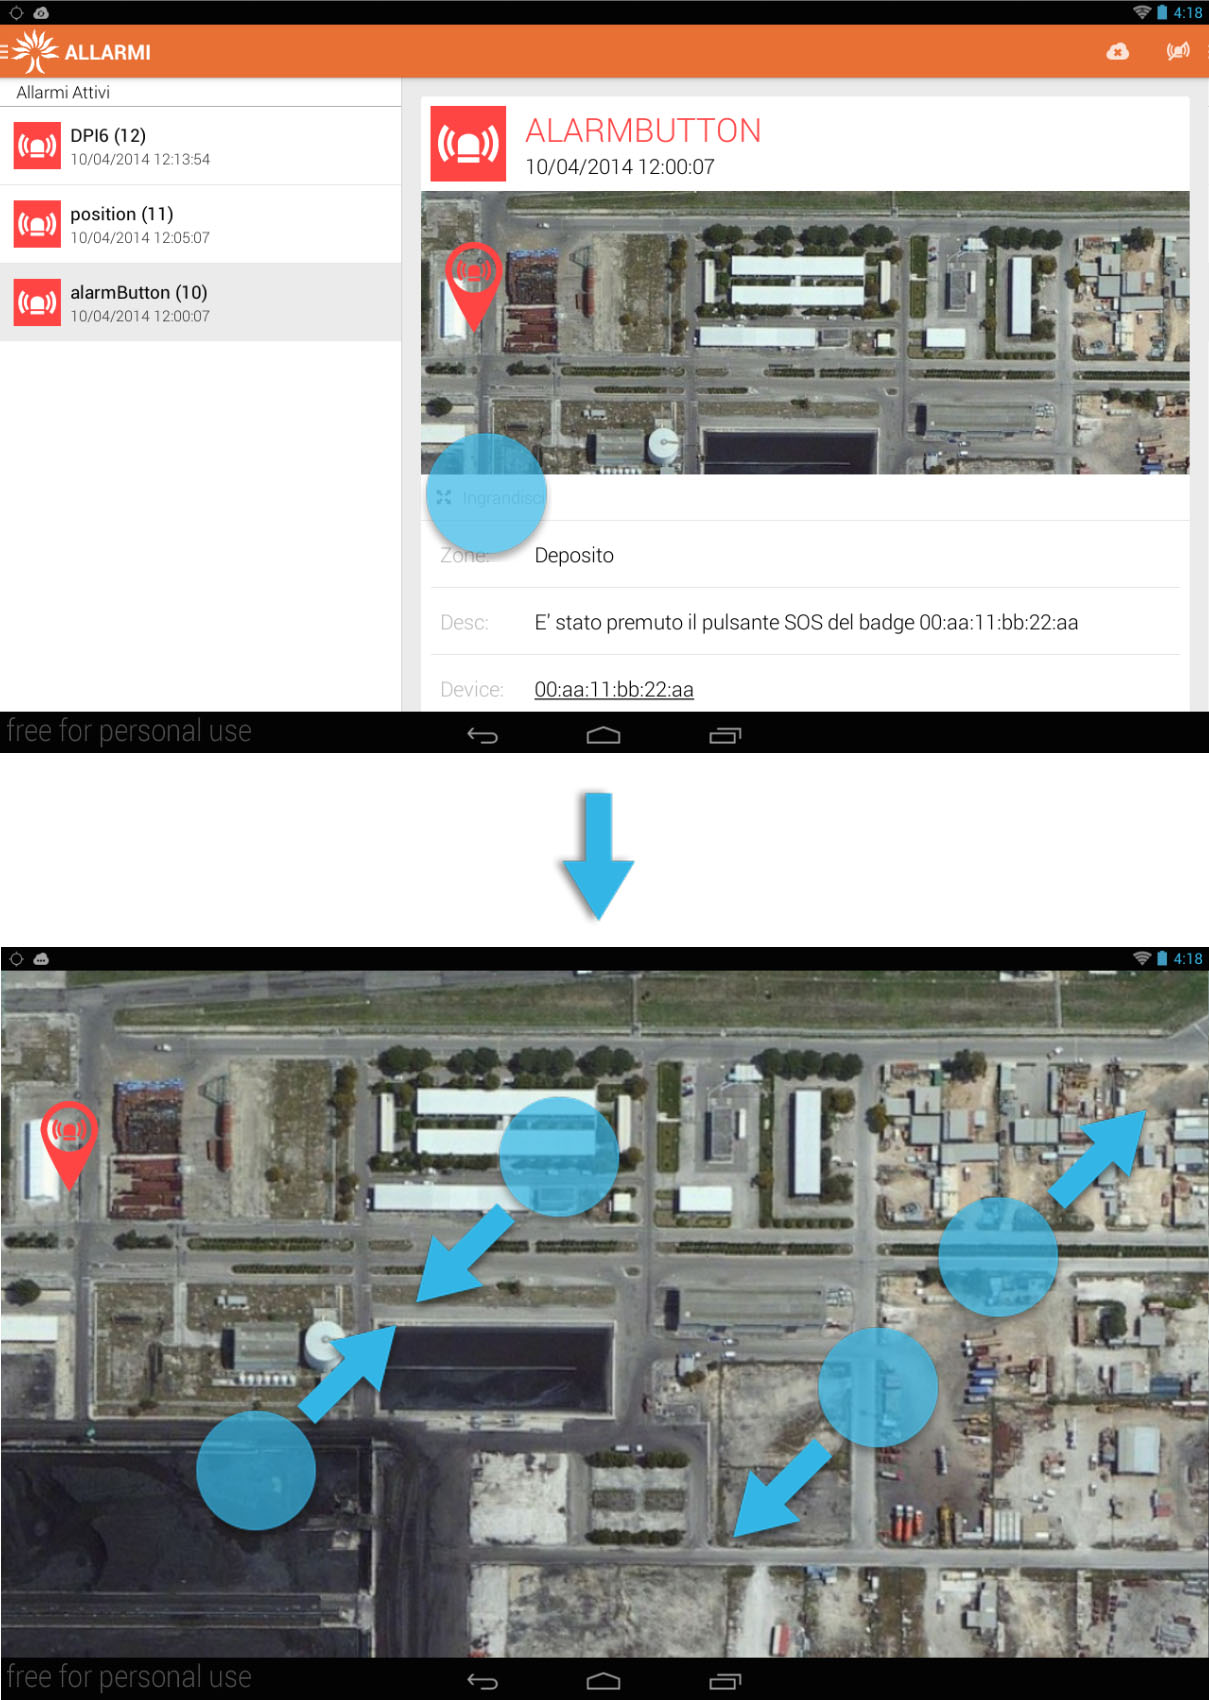
\includegraphics[width=1\textwidth, angle=0]{tablet_allarme_map.jpg}}
		  \caption{Tablet - Map zoom}
	\end{figure}

	\begin{figure}[h!]
		  \centering
		    \centering{%
		      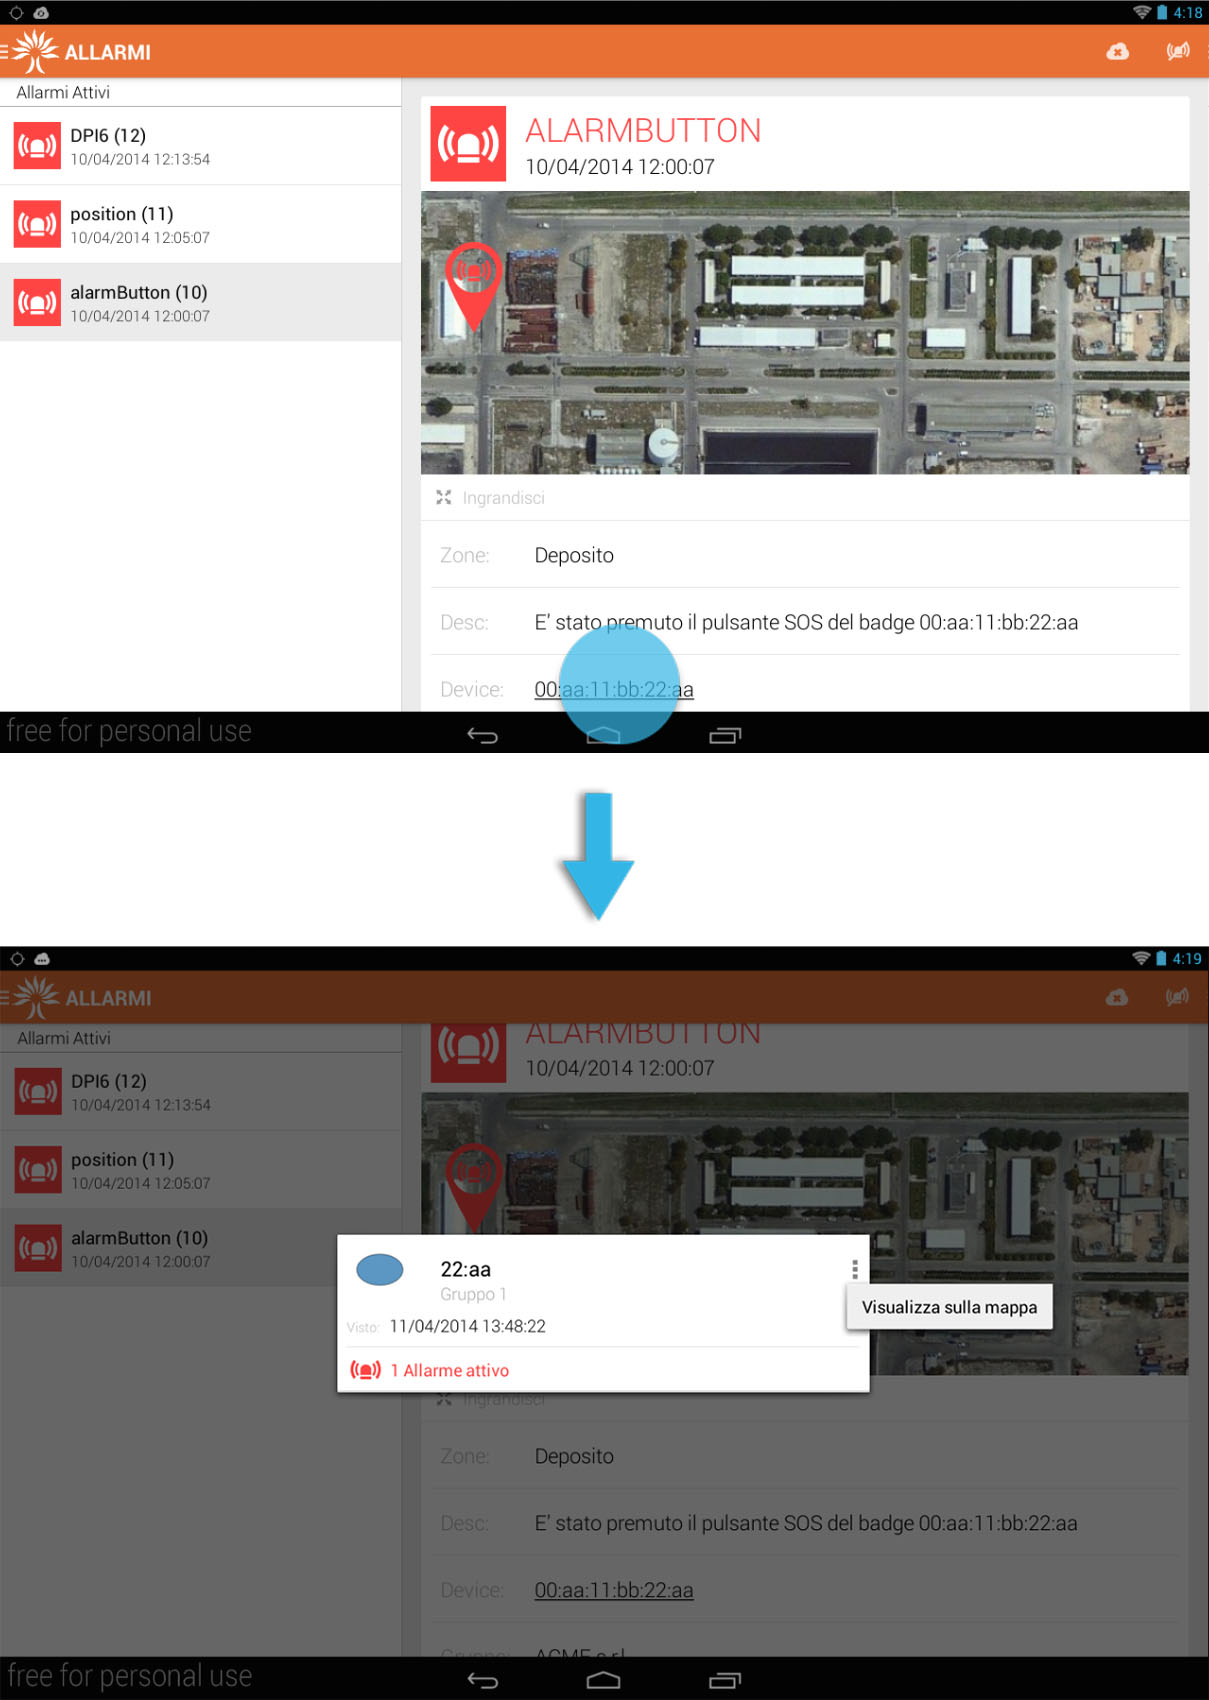
\includegraphics[width=1\textwidth, angle=0]{tablet_allarme_device.jpg}}
		  \caption{Tablet - device details}
	\end{figure}